\section{Dwi Yulianingsih(1174009)}
\subsection{Instalasi Map Server}
\begin{enumerate}
    \item Download terlebih dahulu map servernya. Untuk webnya bisa \href{https://mapserver.org/}{Klik disini} atau \href{https://ms4w.com/}{Klik disini} Untuk windows.
    \hfill\break
    \begin{figure}[H]
		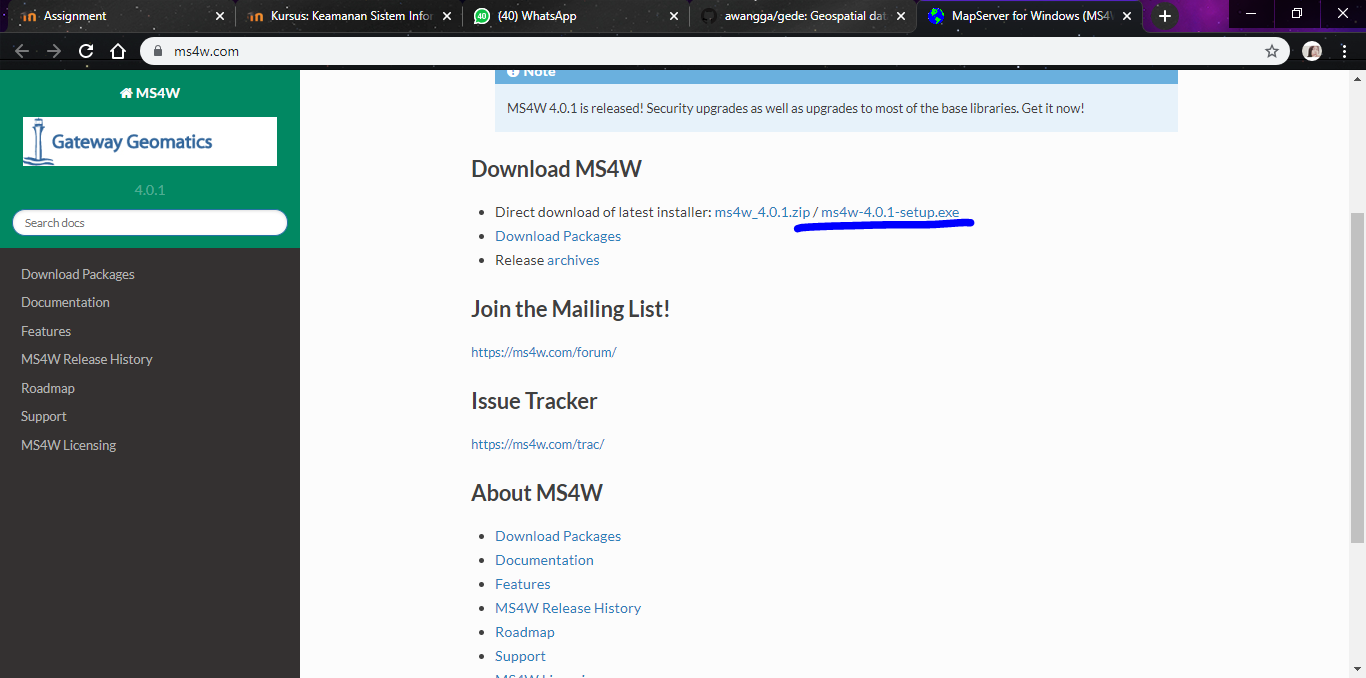
\includegraphics[width=4cm]{figures/1174009/4/1.png}
		\centering
		\caption{Halaman map server untuk windows}
    \end{figure}
   
    \item klik 2 kali pada installer nya
    \hfill\break
    \begin{figure}[H]
		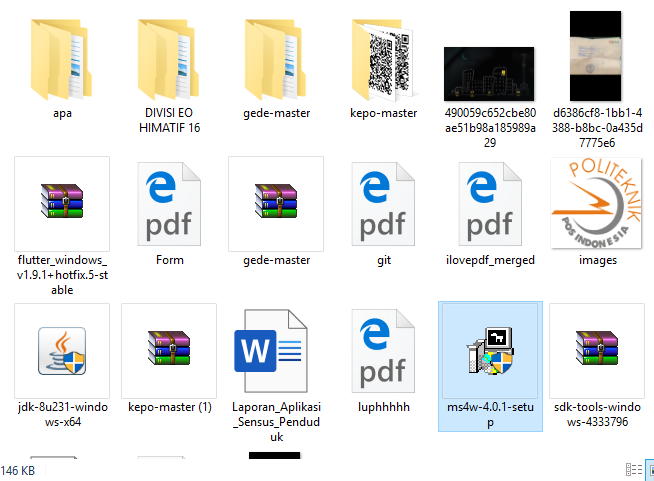
\includegraphics[width=4cm]{figures/1174009/4/2.png}
		\centering
		\caption{klik}
    \end{figure}
 
    \item klik i agree
   \begin{figure}[H]
		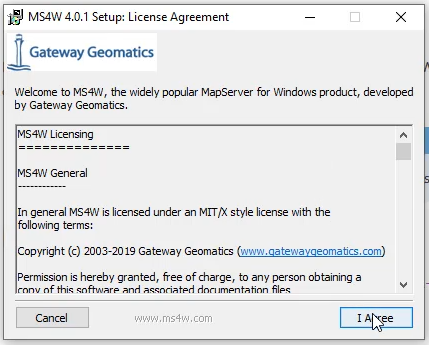
\includegraphics[width=4cm]{figures/1174009/4/3.png}
		\centering
		\caption{klik}
    \end{figure}

 \item pilih tipe installasi yang full
   \begin{figure}[H]
		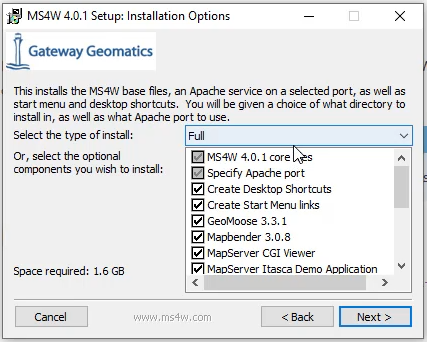
\includegraphics[width=4cm]{figures/1174009/4/4.png}
		\centering
		\caption{full}
    \end{figure}

 \item pilih direktori instalasinya kmeudian next
   \begin{figure}[H]
		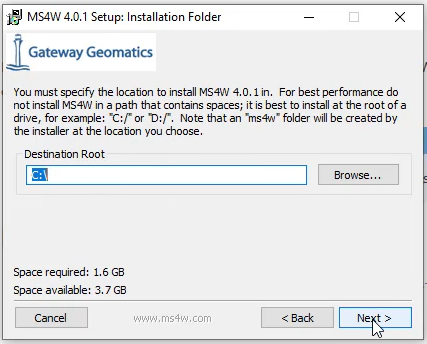
\includegraphics[width=4cm]{figures/1174009/4/5.png}
		\centering
		\caption{pilih}
    \end{figure}

 \item isi port apache yang akan dipakai kemudian next
   \begin{figure}[H]
		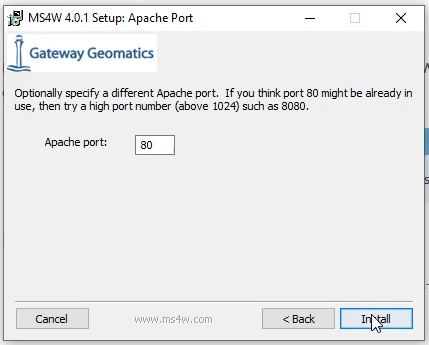
\includegraphics[width=4cm]{figures/1174009/4/6.png}
		\centering
		\caption{apache}
    \end{figure}

 \item tunggu hingga selesai
   \begin{figure}[H]
		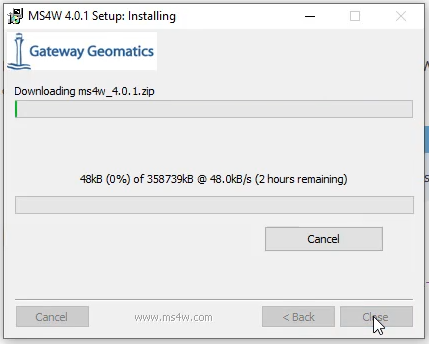
\includegraphics[width=4cm]{figures/1174009/4/7.png}
		\centering
		\caption{klik}
    \end{figure}

 \item klik close
   \begin{figure}[H]
		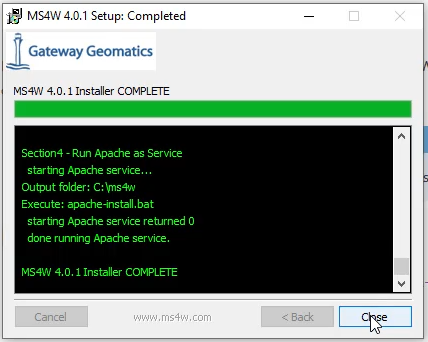
\includegraphics[width=4cm]{figures/1174009/4/8.png}
		\centering
		\caption{tutup}
    \end{figure}

\end{enumerate}

\subsection{Hasil}
\begin{itemize}
\item untuk hasil percobaannya dapat dilihat di yutub dan gambar hasilnya adalah sebagai berikut.
  \begin{figure}[H]
		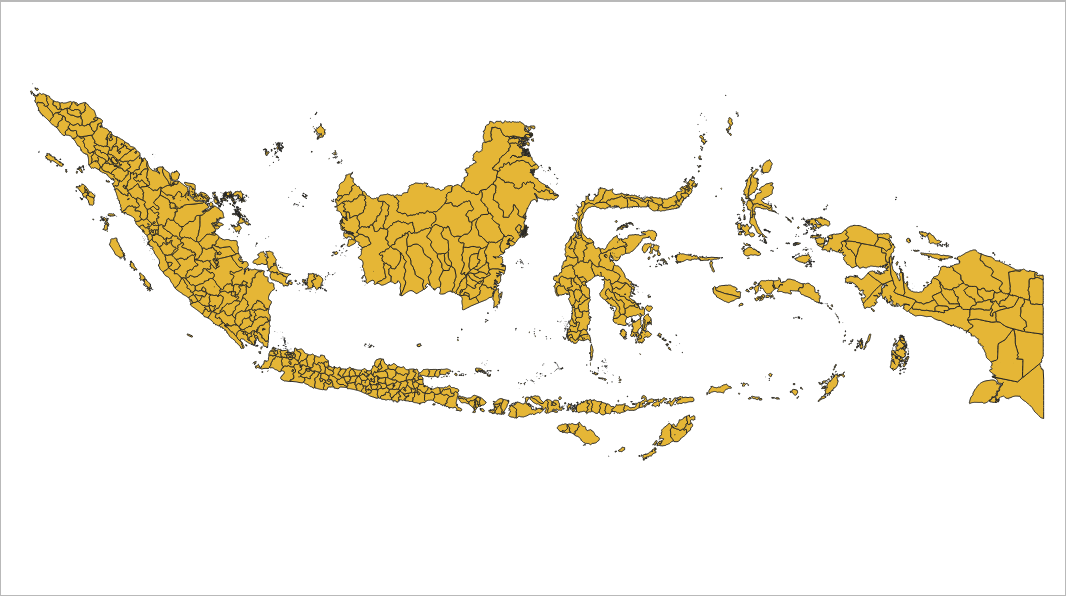
\includegraphics[width=4cm]{figures/1174009/4/gis.png}
		\centering
		\caption{hasil}
    \end{figure}
\end{itemize}


\subsection{Link Youtube}
\href{https://youtu.be/FNY0D3eaa2w}{Klik disini}